\documentclass{article}

% if you need to pass options to natbib, use, e.g.:
% \PassOptionsToPackage{numbers, compress}{natbib}
% before loading nips_2018

% ready for submission
%\usepackage{nips_2018}

% to compile a preprint version, e.g., for submission to arXiv, add
% add the [preprint] option:
\usepackage[preprint]{nips_2018}

% to compile a camera-ready version, add the [final] option, e.g.:
%\usepackage[final]{nips_2018}

% to avoid loading the natbib package, add option nonatbib:
% \usepackage[nonatbib]{nips_2018}

\usepackage[utf8]{inputenc} % allow utf-8 input
\usepackage[T1]{fontenc}    % use 8-bit T1 fonts
\usepackage{hyperref}       % hyperlinks
\usepackage{url}            % simple URL typesetting
\usepackage{booktabs}       % professional-quality tables
\usepackage{amsfonts}       % blackboard math symbols
\usepackage{nicefrac}       % compact symbols for 1/2, etc.
\usepackage{microtype}      % microtypography
\usepackage{tikz}

\title{Sentiment Analysis: Predicting Yelp Scores with BERT}

% The \author macro works with any number of authors. There are two
% commands used to separate the names and addresses of multiple
% authors: \And and \AND.
%
% Using \And between authors leaves it to LaTeX to determine where to
% break the lines. Using \AND forces a line break at that point. So,
% if LaTeX puts 3 of 4 authors names on the first line, and the last
% on the second line, try using \AND instead of \And before the third
% author name.

%TODO: turn off anonymous mode

\author{
  Lichen Zhang (lichenz)\\
  Carnegie Mellon University\\
  Pittsburgh, PA 15213 \\
  \texttt{lichenz@andrew.cmu.edu} \\
  \And
  Jinyao Zhang (jinyaoz)\\
  Carnegie Mellon University \\
  Pittsburgh, PA 15213 \\
  \texttt{jinyaoz@andrew.cmu.edu} \\
  \AND
  Pengtao Ni (pni)\\
  Carnegie Mellon University \\
  Pittsburgh, PA 15213 \\
  \texttt{pni@andrew.cmu.edu} 
}

\begin{document}
% \nipsfinalcopy is no longer used

\maketitle

\begin{abstract}
  Understanding the sentiment behind a text is a challenging task for machines. Given the user review data from Yelp, we explore multiple ways to build models that predict the score of the reviews and understand the factors that make a review positive or negative. By using the state-of-art natural language understanding model \textbf{BERT}, we are able to achieve a testing accuracy of 62\% which is 50\% higher than a baseline $L_1$ regression approach, which is only around 40\% accuracy.
\end{abstract}

\section{Introduction}

Natural language processing is one of the most important applications of machine learning. There has been multiple pre-trained language models that are able to perform different natural language understanding text, including the word-level interpretation models such as Word2vec (Tomas Mikolov, et al. 2013)\cite{3}
and Glove (Jeffrey Pennington, et al. 2014)\cite{4}
 and the sentence-level recognition models such as BERT, which stands for Bidirectional Encoder Representations from Transformers (Jacob Devlin, et al. 2018)\cite{2}. \\
 
Understanding the sentiment behind a text has been a particularly challenging task, since there are no explicit metrics that determine or classify human sentiment. However, it is crucial to understand the meaning conveyed by the text, which requires an understanding of not only words and tokens but also the underlying structures and tones of the text. \\
 
Our goal essentially consists of two tasks: the first one is to train a model that predicts the ratings (ranging for 1 to 5) of individual yelp reviews based on the numerical features and the review texts; and the second task is to identify the strongest indicators among all the features that leads to either positive or negative ratings. Our training and testing data both include the review text and classified features such as date, usefulness score (ranging from 1 to 5), restaurant name, restaurant location (represented by longitude and latitude), etc. Readers may find more information about our dataset in the dataset section. \\

\section{Background and related works}

\subsection{$L_1$ Regularization}
Regularization is an old but useful idea. The intuition behind is to do model
selection by restricting the parameter of models being too large. There are
many types of regularization, the most popular family is the $\ell_p$ norm 
regularization family. In this work, $L_1$ regularization has been applied,
which guarantees a better convergence rate than $L_2$ regularization or
non-penalization setting, if the given model assumption is correct. Moreover,
$L_1$ regularization can be used as a tool of feature selection ---- in 
first-order based convex optimization, adding $L_1$ regularization 
encourages the model to ``shrink'' insignificant weights to 0, which can be
viewed as a tool that combines training and feature selection. (Andrew Ng,
2004)\cite{1}.

\subsection{BERT}
BERT, which is the abstraction of Bidirectional Encoder Representation from Transformers, is the state-of-the-art sentence-level language understanding model . It is designed to "pre-train deep bidirectional representations from unlabeled text by jointly conditioning on both left and right context in all layers" (Jacob Devlin, et al. 2018)\cite{2}. \\

There are two steps in the BERT framework: pre-training and fine-tuning. In the pre-training step, BERT first masks some tokens at random and then trains a bidirectional language model to predict these masked tokens with a deep learning architecture of 12 layers and 768 hidden states. Then it strengthens the model with the \textit{next sentence prediction}(NSP) task. To perform downstream language processing tasks such as question-answering and language classification, BERT plugs in the task-specific inputs and outputs and fine-tune all the parameters end to end. Only the last layer of the model is task-specific, thus fine-tuning pre-trained BERT is not as costly.\cite{2}\\

\subsection{GloVe}
Glove is a pre-trained vector space representations of words combining the advantages of both global matrix factorization and local context window methods. The representation model is trained only on the nonzero elements in a word-word covariance matrix, which leads to a high performance on word analogy tasks. It also provides an accurate prediction on word similarity tests. (Jeffrey Pennington, et al. 2014)\cite{4}.

\section{Methods}
We adapt slightly different methods for the two tasks: feature significance analysis and predictor model training. However, BERT is involved in both tasks as we try to improve on the baseline approach. \\

\begin{figure}
\begin{center}
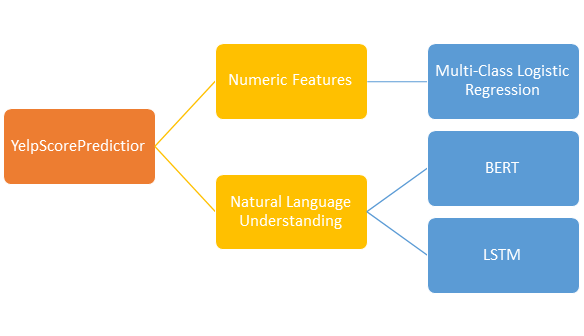
\includegraphics[scale=0.5]{approach_outline}
\caption{Approach Outline}
\end{center}

\end{figure}






\subsection{Feature Significance Analysis}
Our baseline model is a linear regression with numerical features, which is everything except the comment text of the review data. The way we perform feature selection is via $L_1$ regularization. We expect the weight of insignificant features to shrink to 0 by $L_1$ regularization. Therefore, we can sort weights based on their norms, to get a ranking of features. To improve on that, we use BERT to generate a word-embedding for sentences. Then combining with numerical features we have used before, we train a final linear layer using this embedding with $L_1$ regularization.

\subsection{Score Predictor}
Baseline model is a simple logistic regression using again numerical features, and our final model is a fine-tuned BERT. More specifically, we first load the pre-trained BERT model, then add up a final linear classification layer, this final layer is what have trained for. We have strong confidence in this learning framework, since in the original paper of BERT, authors achieve very high accuracy using this fine-tuned strategy.

\section{Dataset}
%TODO: how to cite this / Do we want to mention this at all?
%Let's put it here, since it's a required section.
Each of our input data contains a variety of features:
\begin{itemize}
	\item Stars - Stars of the review (1=worst, 5=best). The value only takes integers between 1 and 5. This is only available in the training data.
	\item ID - Id number of the review. This is only available in the testing and
	validation data.
	\item Name - Name of the business
	\item Text - Review Text
	\item Date - Date of Review
	\item Useful - Number of Yelp users who thought the review was useful. This
	value takes whole numbers (i.e. 0,1,2,...)
	\item Funny - Number of Yelp users who thought the review was funny. This
	value takes whole numbers (i.e. 0,1,2,...)
	\item Cool - Number of Yelp users who thought the review was cool. This value
	takes whole numbers (i.e. 0,1,2,...)
	\item City - City in which the business is located
	\item Longitude - The business’s longitude location
	\item Latitude - The business’s latitude location
	\item Categories - An un-parsed string that categorizes the businesses into Yelp’s categories.
	\item nchar - Number of characters in the review
	\item nword - Number of words in the review. The word count only considers
	words that are not part of the list in stop words (e.g. “a”,”I”,”the”,etc.),
	which is part of the R package tidytext.
	\item Sentiment Score - A score of the text’s sentiment using the AFINN lexicon, which ranges from -5 (very negative) to 5 (very positive).
	\item Gem - Number of times the word “gem” appears in the review text.
	\item Incredible - Number of times the word “incredible” appears in the review
	text.
	\item Perfection - Number of times the word “perfection” appears in the review
	text.
	\item BLANK - Number of times the word “BLANK” appears in the review
	text.
\end{itemize}

We partitioned the features into two classes - we call all the features besides the Text "numerical features" as they could be represented by numbers or discrete classes. For those features that are not represented by numbers, such as Category, we pre-process the data by assigning a number to each category and mapping the features to their numerical representations. In our baseline approach, we only used the numerical features to train the models. When we incorporated the text into the feature, we experimented with two pre-processing methods: using GloVe to represent each word in the text, and using BERT to generate an embedded model of the text. 

\section{Experiments and Results}
Due to time constraint, we didn't finish the LSTM model with GloVe 
embedding, so the below discussions will focus on baseline models and 
BERT.
\subsection{Feature Analysis}
\subsubsection{Baseline: $L_1$ regularization}
Since BERT is a strong and robust pre-trained model, we won’t add a lot more complexity to our final model, as using a simpler model would drastically increase the interpretability of the results. Thus, we propose using linear model for ease of interpretation. For feature selection, we use linear regression with $L_1$ regularization, this combines training together with feature selection.  Intuitively, $L_1$ regularization will pull the weights of useless features to 0, therefore, we can select features based on the weights of their norms.\cite{1} \\

Our baseline for this problem is a simple linear regression with $L_1$ regularization, using only numerical features. This model achieves a 1.77 mean squared error on test dataset. We then use only top 10 features ranked by the norm of weights, this gives a 1.81 test loss.

\subsubsection{Using Pre-trained BERT Model}
 We feed review text into pre-trained BERT and use its last hidden states as our representation of text. Using purely BERT processed text, we get loss down to 1.42. Combining features in baseline and BERT, we finally get shrink loss to 1.35, which beats all our previous models. We validate the effectiveness by selecting top 100 features, and this model gives a loss of 1.41. See \ref{fig2} for more details.
\begin{figure}
\label{fig2}
\begin{center}
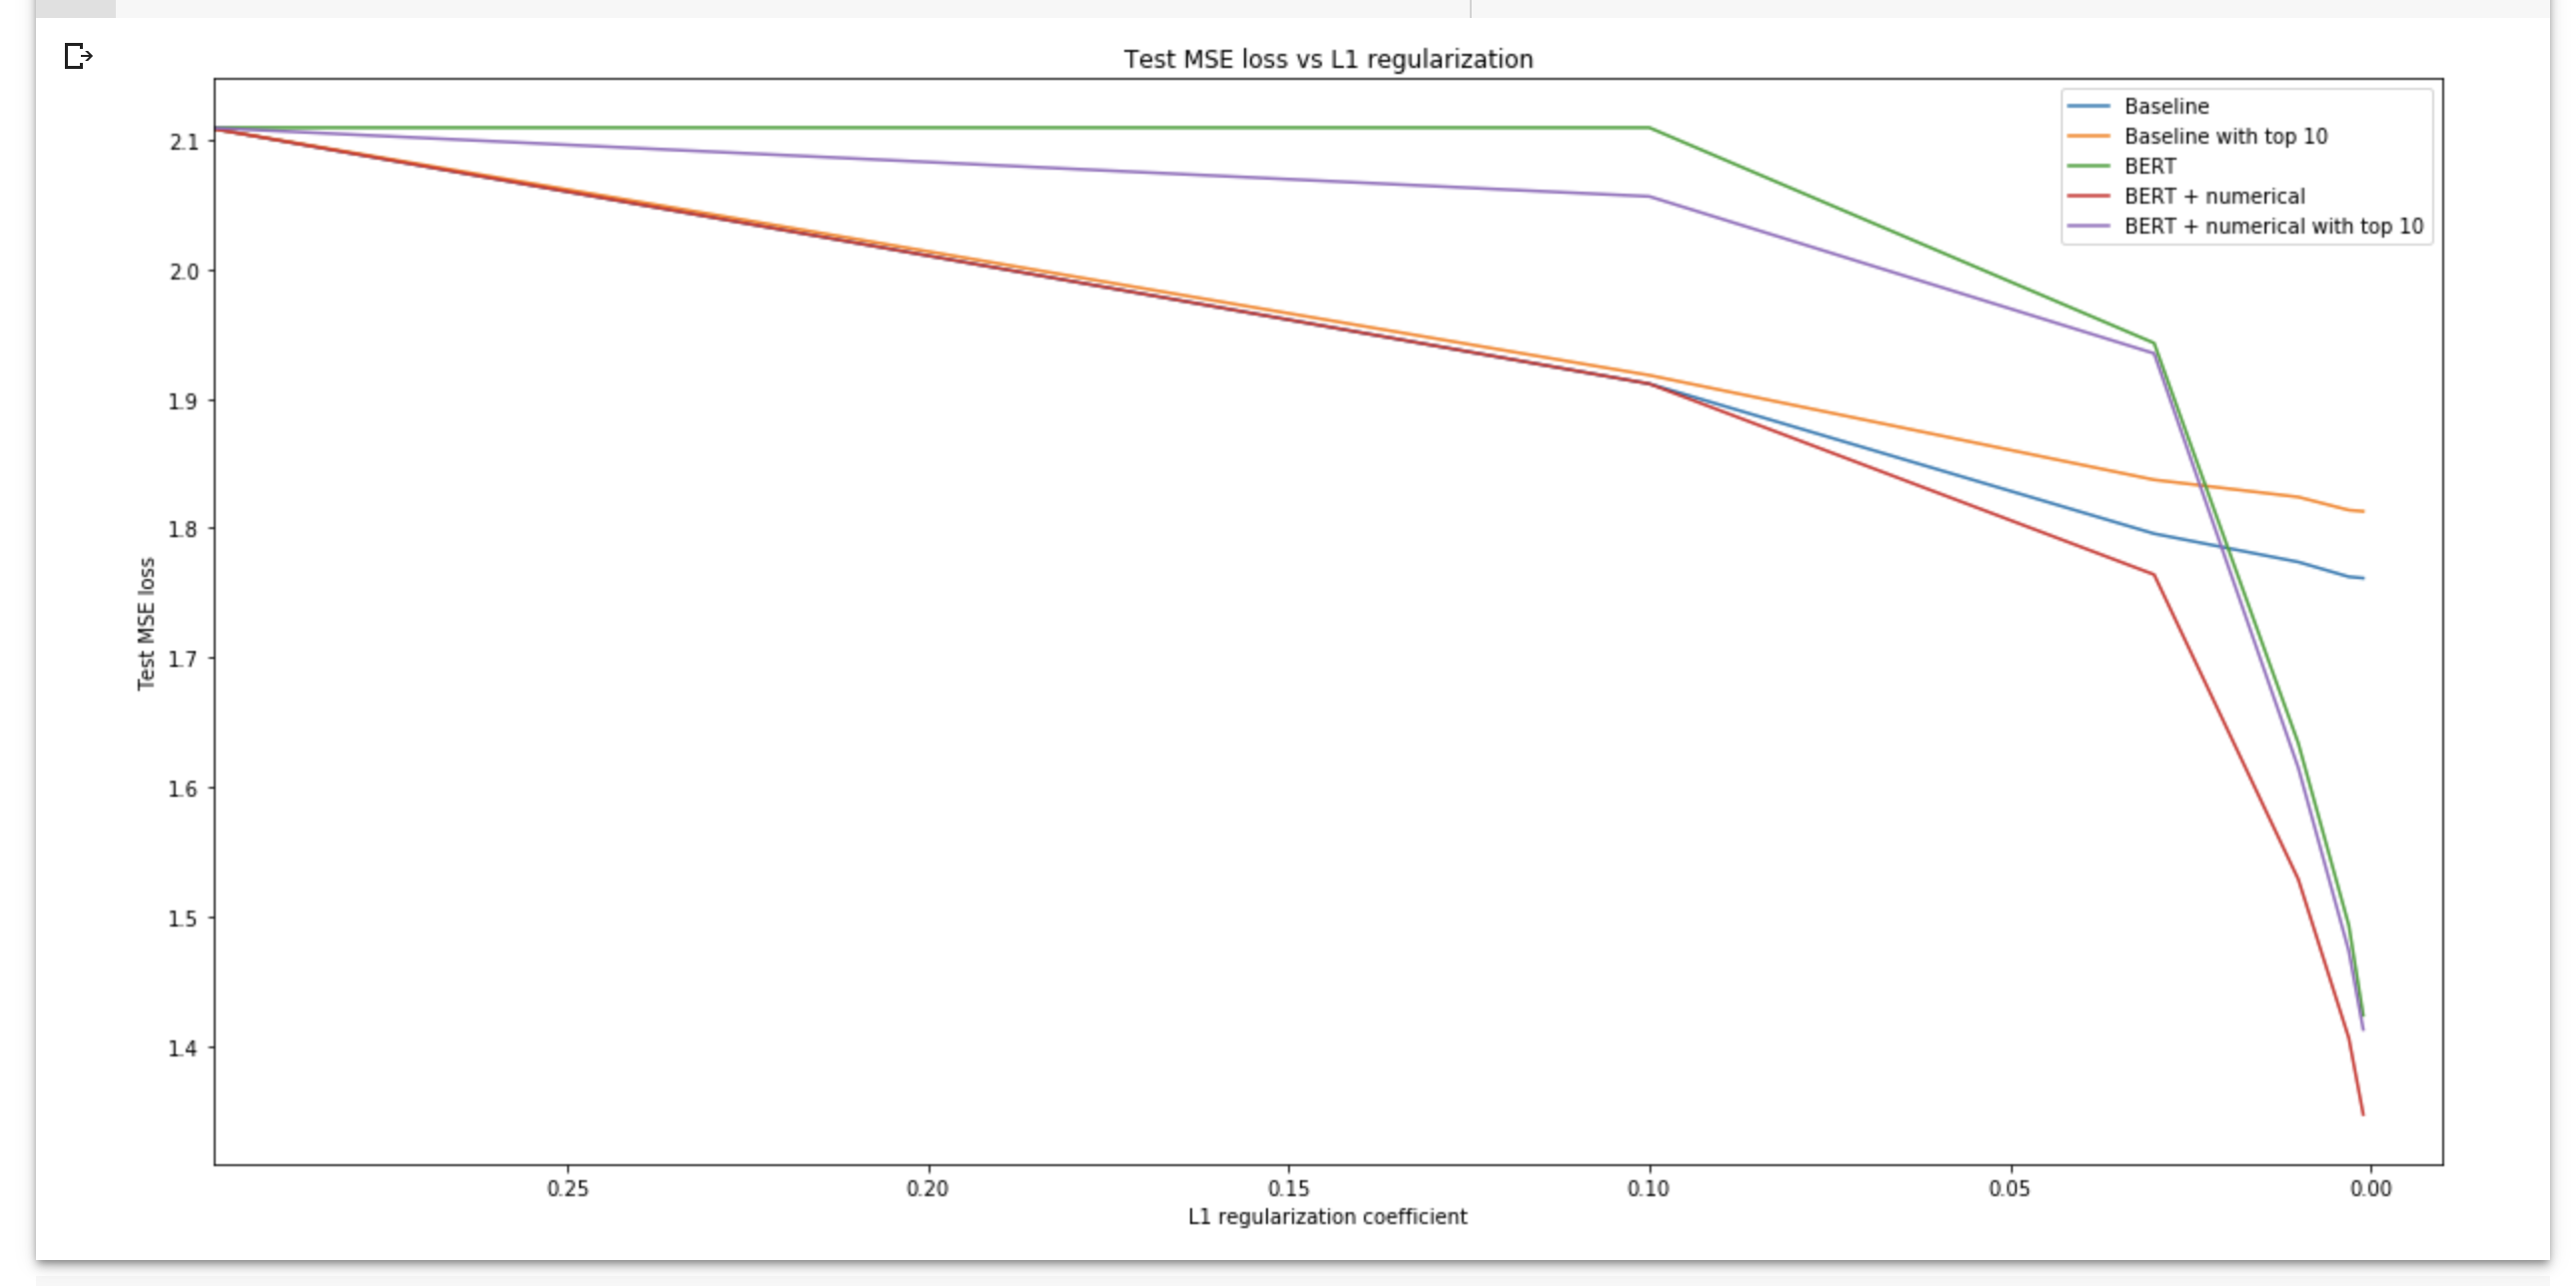
\includegraphics[scale=0.3]{mse_loss_vs_l1}
\caption{Mean-squared error with respect to $L_1$ regularization coefficient}
\end{center}
\end{figure}

\subsubsection{Analysis and Adjustments}
\begin{figure}
\begin{center}
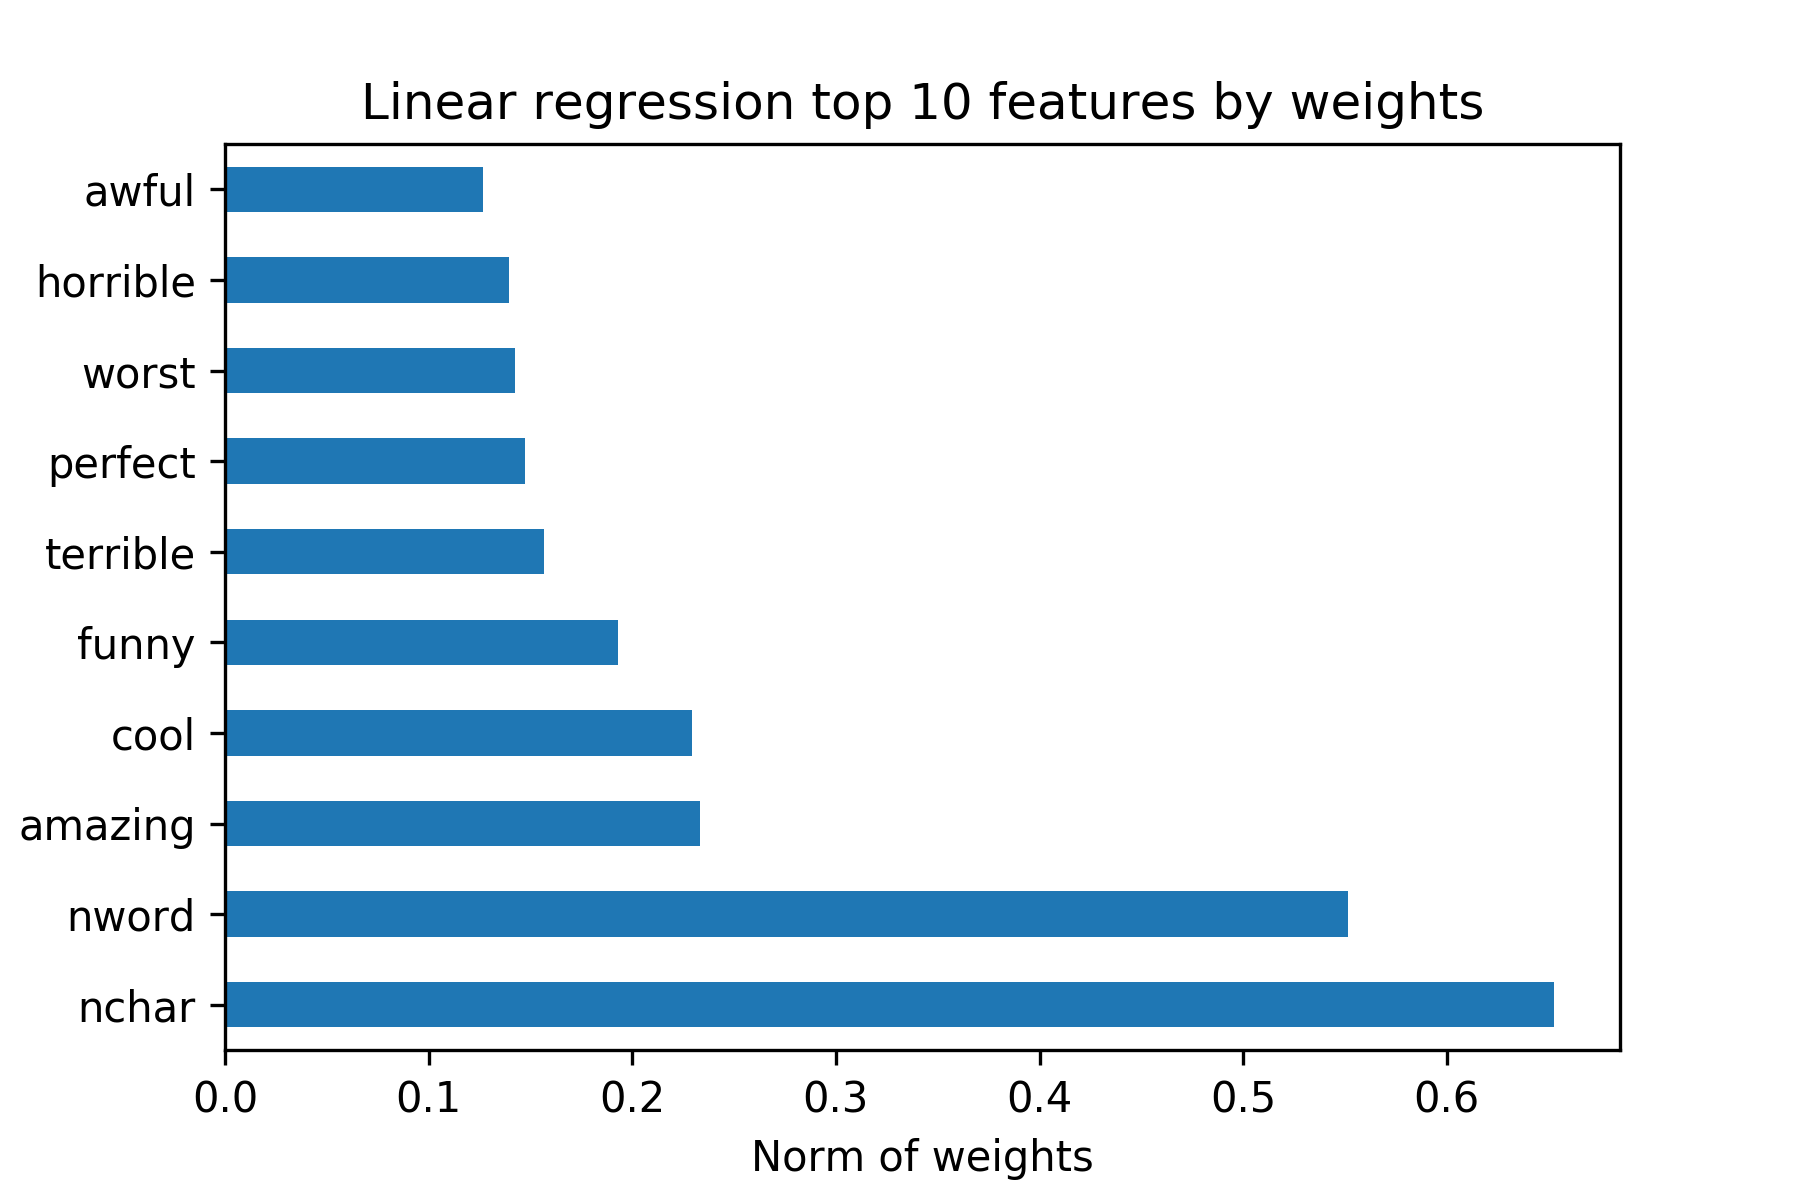
\includegraphics[scale=0.6]{top_10_linear}
\caption{Top 10 features selected by baseline}
\end{center}
\end{figure}
It is worth noting that \texttt{nchar} and \texttt{nword} are ranked highest by
their weights, which is in contrast of what we have thought about. We 
expect words that indicate strong positive or negative sentiment to have
higher weights, which is not the case in the baseline model. \\

When using BERT, we expect the expressiveness of BERT will give a good
representation of words and sentences, therefore, some features in that
have high rank in baseline will be ``washed out''. See \ref{fig4} for a 
comparison.
\begin{figure}
\begin{center}
\label{fig4}
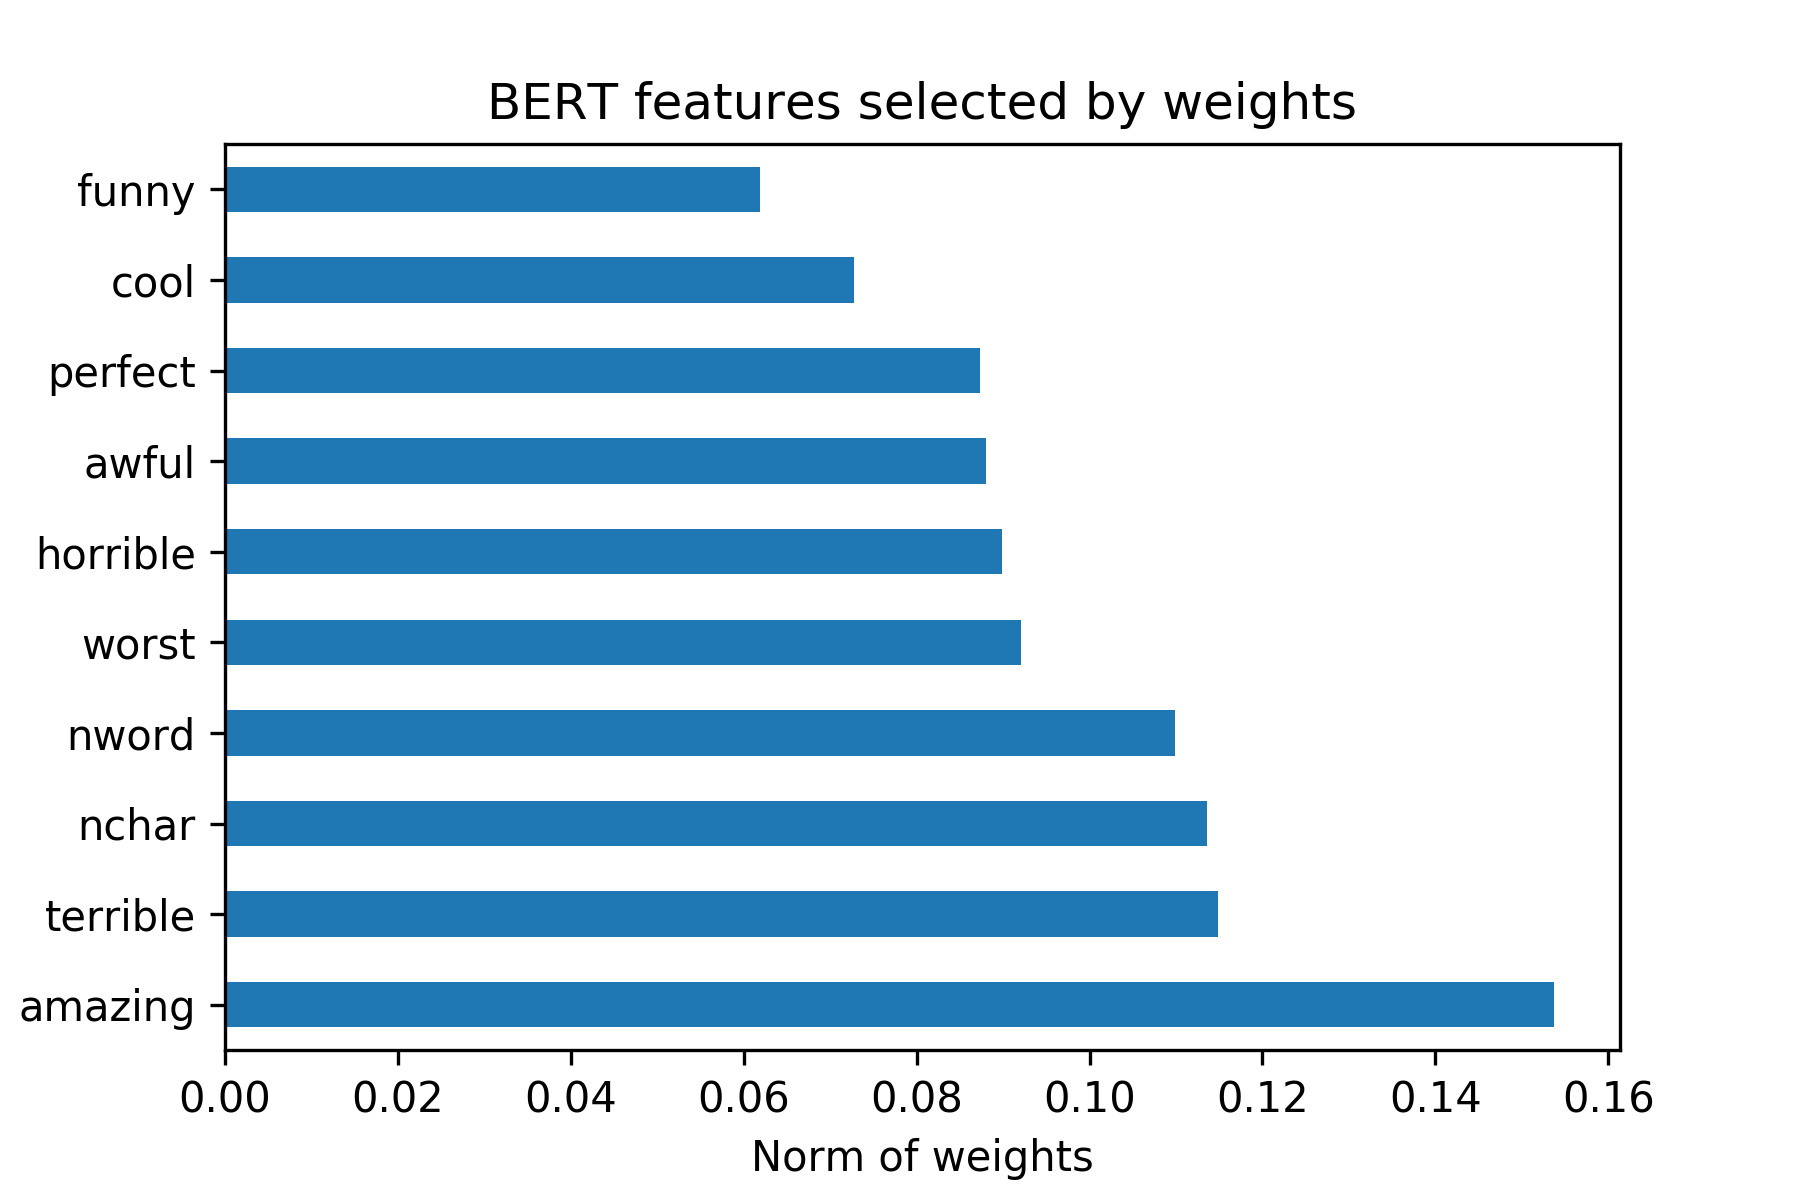
\includegraphics[scale=0.6]{top_10_bert}
\caption{Top 10 numerical features selected by BERT-based model}
\end{center}
\end{figure}
The first observation is the norm of weights have decreased drastically. This
reflects our expectation, since BERT is more expressive than these numerical
features, the contribution of numerical features have been significantly 
reduced. In our final BERT model, we have $768+35=803$ features, among
the top 100 features, only 1 numerical feature appears, namely, the 
occurrence of word \texttt{amazing}. On the other hand, for the top 200
features, 33 numerical features have appeared, which means we haven't
completely washed them out via BERT embedding. 
\subsection{Predicting Scores}
\subsubsection{Baseline: Logistic regression}
In score-predicting task, our baseline model consists of a simple logistic 
regression using only numerical features. Main advantage of this simple
model is, training is lightning fast, therefore, we can perform more 
comprehensive and sophisticated model selection by cross-validation, which
is intrinsically hard for deep and complex models. With 10-fold 
cross-validation, we get an accuracy around 40\%.

\subsubsection{Fine-tuning Pre-trained BERT model}
We adapt the strategy described in \cite{2}, by adding an extra linear layer
to the pre-trained BERT model, and final training mainly involves training the
parameters of last layer. Error still got propagated back to the entire model,
but major learning happens only in the last layer, so fine-tuning process is
much faster than training the entire model. In our experiment, it takes around
50 minutes to train an epoch of our dataset, which compromised of around
30000 sentences. Final accuracy of this model is around 62\%. We refer 
readers to \ref{fig5} for figures.
\begin{figure}
\label{fig5}
\begin{center}
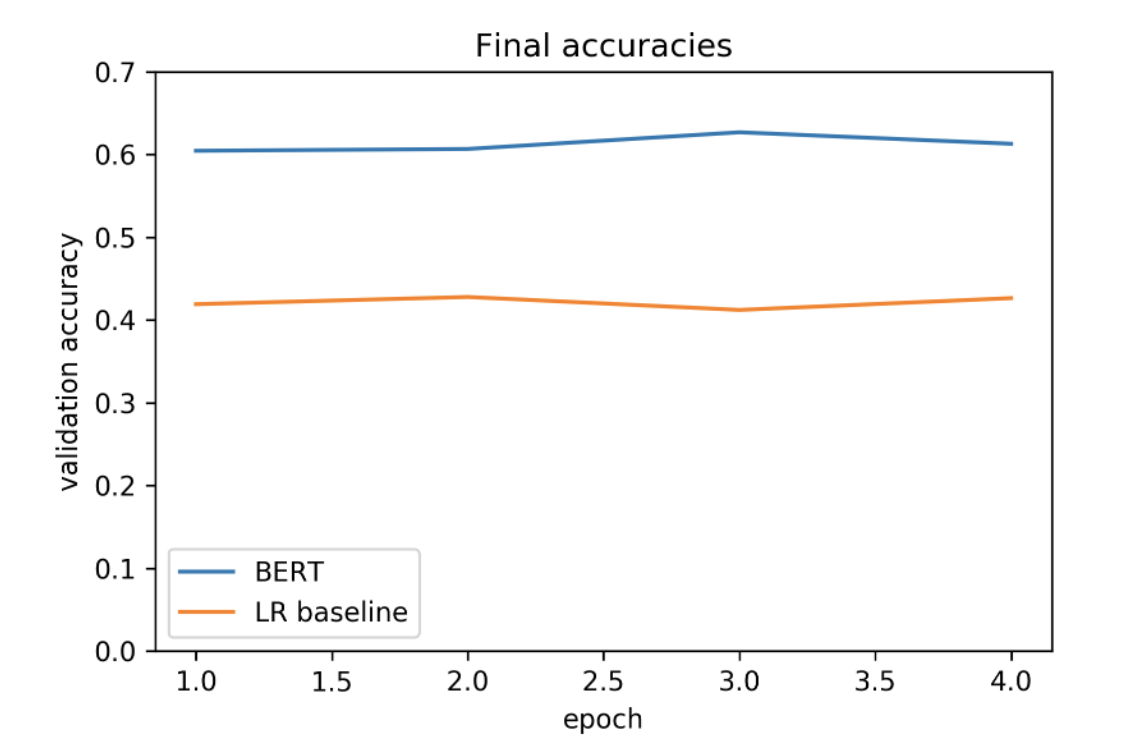
\includegraphics[scale=0.6]{final_acc}
\caption{Final accuracy of predicting scores}
\end{center}
\end{figure}

\subsubsection{Analysis and Adjustments}
As the state-of-the-art natural language understanding model, BERT 
outperforms baseline model to a significant extent. However, it is worth 
noting that such accuracy has not yet achieved the performance of BERT on
other sentiment analysis task. For example, in Netflix review prediction, 
BERT achieves an accuracy over 95\%. One phenomenon we have observed
is, BERT generally performs well when output is binary, i.e., in task like 
classifying whether a review is positive or not. Additionally, we measure the
accuracy by using a 0-1 loss, i.e., if prediction matches output label, we give
a 1, otherwise 0. Due to the structure of this specific task, it might be 
better to use more sensitive measurement of loss.

\section{Conclusion and Future Work}
\subsection{Conclusion}

%TODO: Review this paragraph
Sentiment analysis and further classification and prediction is a non-trivial task. One key component is how to feature engineer the text into features, in order to address this problem, we make use of the state of the art natural language understanding model, BERT, which generates an embedding for sentence. This pre-trained fine-tuned model proves to be useful for both tasks ---- in sentiment score regression problem, it reduces 30\% loss compared to baseline model. For classifying star ratings, it improves 50\% accuracy compared to baseline. Also, $L_1$ regularization proves to be a useful feature selection tool. \\

\subsection{Reflections and Future Work}
One might notice that, even though we are able to achieve a significant improvement over the baseline approach, a final testing accuracy of 62\% is still far from optimal. One possible reason is labels of data are very imbalanced: one third of them are 4, one third of them are 5, and only one third are 1,2 and 3. We haven’t found a way to address this problem. One possibility is to augment the labels using some generative way: for example, interpolate the data points, then using KNN to generate some similar data. The other is switch to some more advanced generative model, such as the SMOTE algorithm\cite{5}. 
 We believe that these pre-processing methods will be able to increase the testing performance. \\

Another issue that we are yet to address is the problem of combining BERT with all the numerical features. We reason that padding a dense layer right before the output layer might be a feasible approach. However, if we simply join the embedded word representations of the text from BERT to the other numeric features in such a linear setting, there might not be a significant difference between this method and our feature analysis model. We might also propagate error back to BERT pre-trained weights. Due to time constraint (training one epoch of BERT takes more than 50 minutes), we don’t have a clear answer to this question. \\





% I left this part intentionally for reference





%TODO: add references
\bibliographystyle{unsrt}
\bibliography{ref}

\end{document}